\documentclass[aspectratio=43,t]{beamer}
%\documentclass[aspectratio=43,t,handout]{beamer}

% Language and General Settings
\usepackage[T1]{fontenc} 				% Umlauts and correct hyphenation
\usepackage[utf8]{inputenc} 			% Unicode t
\usepackage{textcomp} 				% Various symbols (e.g. �, �) 
\usepackage{amsmath}				% Math environment
\usepackage{mathtools}				% Math environment for curly brackets
\usepackage{bm}					% Boldface inside math environment
\usepackage{amssymb} 				% Various mathematical symbols
\usepackage{hyperref} %\usepackage[hidelinks]{hyperref}			% Links within document not labeled
\usepackage[final]{microtype}			% Better justification
\usepackage{color}					% Enables definition of own colors

% Listings
\usepackage{listings} 					% Program code environment
\lstset{
	language=C++, 
	showstringspaces=false,
	breaklines=true,
	basicstyle=\tiny\ttfamily,
	keywordstyle=\color{blue},
	stringstyle=\color{red},
	commentstyle=\color{green},
	morecomment=[l][\color{magenta}]{\#},
	title=\lstname}

% Images/ Plots
\usepackage{pgfplots}					% Enables including of tikz-images
\usetikzlibrary{calc}
\pgfplotsset{compat=newest}%
\pgfplotsset{table/search path ={../}}		% Search path for data is lowest directory now
\newlength\figureheight 				% Command to adjust the size of pgf-plots
\newlength\figurewidth
\usepackage{graphicx}					% Enables including of various graphics formats
\usepackage{caption}					% Enables including of various graphics formats
\usepackage{subcaption}				% Enables subfigures
\usepackage{chngcntr}				% Continuous numbering of images
\usepackage{epstopdf}				% Enables including of eps-images
\graphicspath{img/}					% Path to images
\usepackage{adjustbox}
\usepackage{smartdiagram}
\usepackage{multimedia}

%English version FAU Logo
\usepackage[english]{babel}
%German version FAU Logo
%\usepackage[ngerman]{babel}
\usepackage[backend=biber,sorting=none,doi=true,style=ieee]{biblatex}

% Themes:
%  - fau:          FAU theme
%  - fau-med:      MedFak FAU theme
%  - fau-nat:      NatFak FAU theme
%  - fau-phil:     PhilFak FAU theme
%  - fau-rw:       RWFak FAU theme
%  - fau-rw-jura:  RWFak FB Jura FAU theme
%  - fau-rw-wiso:  RWFak FB WISO FAU theme
%  - fau-tf:       TechFak FAU theme
%
% Options:
%  - image:        Cover image on title page
%  - plain:        Plain title page
%  - longtitle:    Title page layout for long title
\makeatletter
  \def\beamer@calltheme#1#2#3{%
    \def\beamer@themelist{#2}
    \@for\beamer@themename:=\beamer@themelist\do
    {\usepackage[{#1}]{\beamer@themelocation/#3\beamer@themename}}}

  \def\usefolder#1{
    \def\beamer@themelocation{#1}
  }
  \def\beamer@themelocation{}

\usefolder{themefau}
\usetheme[longtitle]{fau-tf}

% Enable semi-transparent animation preview
\setbeamercovered{transparent}

\defbibheading{bibliography}{}
\addbibresource[label=primary]{literature.bib}

\usepackage{csquotes}																% Avoids warning when using BibLaTeX
\usepackage[noabbrev]{cleveref}																% Have automatic formatting of references: use \cref or \Cref{labellist} instead of \ref 
%\crefname{section}{}{}
\usepackage{siunitx}														% format SI units
\usepackage{smartdiagram}

% Title, authors, and date
\title{From Cellular Automata \\to the Lattice Boltzmann Method}
\author[T. Pollinger, M. Gaißert]{Theresa Pollinger, Marcial Gaißert}
\institute[Ferienakademie 2017]{Ferienakademie Sarntal 2017}
\date{\today}
% Setting right internal properties for the pdf-file
\usepackage{ifpdf}
\ifpdf
\hypersetup{pdfauthor={Theresa Pollinger, Marcial Gaißert}}
\hypersetup{pdftitle={From Cellular Automata to the Lattice Boltzmann Method}}
\fi

% Additions for cellular automata
\newlength\cacellsize

\begin{document}
% Title
\maketitle

  { % Outline
    \setbeamertemplate{footline}{}
    \begin{frame}[noframenumbering]{Outline}
      \tableofcontents
    \end{frame}
  }
 
%TODO an Julian schicken, damit er nochmal drüberschaut - Eher an Michael Lahnert, oder?
%- Intro: game of life video (because looks cool)? - like
%- Zelluläre Automaten (5 min)
%- Wie funktioniert/was ist? Beispiel, Vor-/Nachteile
%- Lattice gases (5 min)
%- Als erste Annäherung an LBM; noch sehr ähnlich zu zellulärem Automat.
%- LBM (10 min)
% - Stream-Collide scheme in graphics (or @Marcial do we get that earlier on?)
% - show the similarity to Boltzmann equation, introduce important moments, show most important collision operators
% - Nondimensionalization



\begin{section}{Cellular Automata}
	\begin{frame}{Cellular Automata}
		\begin{columns}
			\column{.4\linewidth}
				\centering
				\begin{itemize}
					\item regular arrangement of cells
					\item<2-> each with discrete state
					\item<3-> updated simultaneously at each step 
					\item<4-> update rules:
					\begin{itemize}
						\item<5-> same for each cell
						\item<6-> only dependent on close-by cells
					\end{itemize}
				\end{itemize}
		
			\column{.6\linewidth}
			\setlength\cacellsize{0.75cm}
			\only<1>{
				\begin{figure}[htbp]
					\centering
					\setlength\figureheight{0.675\textheight}
					\setlength\figurewidth{\figureheight}
					\resizebox{\figurewidth}{\figureheight}{
 \begin{tikzpicture}
    \clip (-1,-1) rectangle (5cm,5cm); % Clips the picture...

    \draw[style=help lines] (-14,-14) grid[step=\cacellsize] (14,14);
  \end{tikzpicture}
}

					\caption*{a grid of cells}
				\end{figure}
			}
			\only<4-6>{
				\begin{table}
					\centering
					\begingroup
					\renewcommand\arraystretch{2}
					\setlength\cacellsize{0.5cm}
					\begin{tabular}{ccc}
						\bfseries previous &\bfseries \#live neighbors &\bfseries next \\\hline\hline
						\raisebox{-1ex}{\Huge$\blacksquare$}
						&$<2$&\raisebox{-1ex}{\Huge$\square$}\\\cline{2-3}
						&$2,3$&\raisebox{-1ex}{\Huge$\blacksquare$}\\\cline{2-3}
						&$>3$&\raisebox{-1ex}{\Huge$\square$}\\\hline
						\raisebox{-1ex}{\Huge$\square$}&$3$&\raisebox{-1ex}{\Huge$\blacksquare$}\\
					\end{tabular}
					\endgroup
					\caption*{Rules of Conway's Game of Life}
				\end{table}
			}
			\only<2-3,7>{
				\begin{figure}[htbp]
					\centering
					\setlength\figureheight{0.675\textheight}
					\setlength\figurewidth{\figureheight}
					\resizebox{\figurewidth}{\figureheight}{
 \begin{tikzpicture}
    \clip (-1,-1) rectangle (5cm,5cm); % Clips the picture...

    \draw[style=help lines] (-14,-14) grid[step=\cacellsize] (14,14);
    \draw [fill=black] (1\cacellsize,2\cacellsize) rectangle (2\cacellsize,3\cacellsize);
    \draw [fill=black] (2\cacellsize,2\cacellsize) rectangle (3\cacellsize,3\cacellsize);
	\draw [fill=black] (3\cacellsize,2\cacellsize) rectangle (4\cacellsize,3\cacellsize);
	\draw [fill=black] (5\cacellsize,4\cacellsize) rectangle (6\cacellsize,5\cacellsize);
  \end{tikzpicture}
}

					\caption*{a grid of cells with state}
				\end{figure}
			}
			\only<8>{
				\begin{figure}[htbp]
					\centering
					\setlength\figureheight{0.675\textheight}
					\setlength\figurewidth{\figureheight}
					\resizebox{\figurewidth}{\figureheight}{
 \begin{tikzpicture}
    \clip (-1,-1) rectangle (5cm,5cm); % Clips the picture...

    \draw[style=help lines] (-14,-14) grid[step=\cacellsize] (14,14);
    \draw [fill=red] (1\cacellsize,2\cacellsize) rectangle (2\cacellsize,3\cacellsize);
    \draw [fill=black] (2\cacellsize,2\cacellsize) rectangle (3\cacellsize,3\cacellsize);
	\draw [fill=red] (3\cacellsize,2\cacellsize) rectangle (4\cacellsize,3\cacellsize);
	\draw [fill=green] (2\cacellsize,3\cacellsize) rectangle (3\cacellsize,4\cacellsize);
	\draw [fill=green] (2\cacellsize,1\cacellsize) rectangle (3\cacellsize,2\cacellsize);
	\draw [fill=red] (5\cacellsize,4\cacellsize) rectangle (6\cacellsize,5\cacellsize);
  \end{tikzpicture}
}

					\caption*{changes in first step}
				\end{figure}
			}
			\only<9>{
				\begin{figure}[htbp]
					\centering
					\setlength\figureheight{0.675\textheight}
					\setlength\figurewidth{\figureheight}
					\resizebox{\figurewidth}{\figureheight}{
 \begin{tikzpicture}
    \clip (-1,-1) rectangle (5cm,5cm); % Clips the picture...

    \draw[style=help lines] (-14,-14) grid[step=\cacellsize] (14,14);
    \draw [fill=black] (2\cacellsize,2\cacellsize) rectangle (3\cacellsize,3\cacellsize);
	\draw [fill=black] (2\cacellsize,3\cacellsize) rectangle (3\cacellsize,4\cacellsize);
	\draw [fill=black] (2\cacellsize,1\cacellsize) rectangle (3\cacellsize,2\cacellsize);
  \end{tikzpicture}
}

					\caption*{after first step}
				\end{figure}
			}
		\end{columns}
	\end{frame}


	\begin{frame}{Cellular Automata -- advantages and disadvantages}
		%TODO some more?
		\centering
		\begin{tabular}{c c}
			\bfseries advantages & \bfseries disadvantages \\\hline
			\begin{minipage}{0.4\linewidth}
				\vspace{1ex}
				\begin{itemize}
					\item<2-> simple structure
					\item<3-> easy to implement
					\item<4-> easy to parallelize
				\end{itemize}
			\end{minipage}
			&\begin{minipage}{0.4\linewidth}
				\vspace{1ex}
				\begin{itemize}
					\item<5-> difficult to design for given macroscopic behavior
				\end{itemize}
			\end{minipage}
		\end{tabular}
	\end{frame}
\end{section}

\begin{section}{Lattice Gas Automata}
	\begin{frame}{Lattice Gas Automata}
		\begin{columns}
			\column{0.4\linewidth}
			\begin{itemize}
				\item Regular arrangement of nodes
				\begin{itemize}
					\item<2-> HPP: square lattice \\$\rightarrow$ does not lead to Navier-Stokes
					\item<3-> FHP: triangular lattice%(Frisch,Hasslacher,Pomeau)
				\end{itemize}
				\item<4-> 6 (7) cells per node
				\begin{itemize}
					\item<4-> one for each direction
				\end{itemize}
				\item<5-> for each step, do:
				\begin{itemize}
					\item<6-> collision
					\item<8-> propagation
				\end{itemize}
			\end{itemize}
			\column{0.6\linewidth}
			\setlength\cacellsize{2cm}
			\only<3>{
				\begin{figure}
					\centering
					\setlength\figureheight{0.675\textheight}
					\setlength\figurewidth{\figureheight}
					\resizebox{\figurewidth}{\figureheight}{
 \begin{tikzpicture}
    \clip (-1,-1) rectangle (5cm,5cm); % Clips the picture...
    
    \coordinate (up) at (0,1*\cacellsize);
    \coordinate (left) at (-0.866*\cacellsize,-0.5*\cacellsize);
    \coordinate (right) at (0.866*\cacellsize,-0.5*\cacellsize);
    
   	\foreach \x in {-7,-6,...,7}{
   		\foreach \y in {-7,-6,...,7}{
   			\coordinate (here) at (1.732*\x*\cacellsize,1*\y*\cacellsize);
   			\draw (here) -- ($(here)+(up)$);
   			\draw (here) -- ($(here)+(left)$);
   			\draw (here) -- ($(here)+(right)$);
   			
   			\coordinate (here) at (1.732*\x*\cacellsize+0.866*\cacellsize,1*\y*\cacellsize+0.5*\cacellsize);
   			\draw (here) -- ($(here)+(up)$);
   			\draw (here) -- ($(here)+(left)$);
   			\draw (here) -- ($(here)+(right)$);
   		}
   	}
  \end{tikzpicture}
}
					\caption*{Triangular lattice}
				\end{figure}
			}
			\only<4-6>{
				\begin{figure}
					\centering
					\setlength\figureheight{0.675\textheight}
					\setlength\figurewidth{\figureheight}
					\resizebox{\figurewidth}{\figureheight}{
 \begin{tikzpicture}
    \clip (-1,-1) rectangle (5cm,5cm); % Clips the picture...
    
    \coordinate (up) at (0,1*\cacellsize);
    \coordinate (left) at (-0.866*\cacellsize,-0.5*\cacellsize);
    \coordinate (right) at (0.866*\cacellsize,-0.5*\cacellsize);
    
   	\foreach \x in {-7,-6,...,7}{
   		\foreach \y in {-7,-6,...,7}{
   			\coordinate (here) at (1.732*\x*\cacellsize,1*\y*\cacellsize);
   			\draw (here) -- ($(here)+(up)$);
   			\draw (here) -- ($(here)+(left)$);
   			\draw (here) -- ($(here)+(right)$);
   			
   			\coordinate (here) at (1.732*\x*\cacellsize+0.866*\cacellsize,1*\y*\cacellsize+0.5*\cacellsize);
   			\draw (here) -- ($(here)+(up)$);
   			\draw (here) -- ($(here)+(left)$);
   			\draw (here) -- ($(here)+(right)$);
   		}
   	}
   
	\node[circle,draw,fill,color=blue,inner sep=2pt] (A) at ($(up)+(right)+0.1*(left)$) {};
	\draw[blue,-latex,thick] (A) -> ($(A)+0.5*(left)$);
	\node[circle,draw,fill,color=blue,inner sep=2pt] (B) at ($(up)+(right)-0.1*(left)$) {};
	\draw[blue,-latex,thick] (B) -> ($(B)-0.5*(left)$);
  \end{tikzpicture}
}
					\caption*{before collision}
				\end{figure}
			}
			\only<7-8>{
				\begin{figure}
					\centering
					\setlength\figureheight{0.675\textheight}
					\setlength\figurewidth{\figureheight}
					\resizebox{\figurewidth}{\figureheight}{
 \begin{tikzpicture}
    \clip (-1,-1) rectangle (5cm,5cm); % Clips the picture...
    
    \coordinate (up) at (0,1*\cacellsize);
    \coordinate (left) at (-0.866*\cacellsize,-0.5*\cacellsize);
    \coordinate (right) at (0.866*\cacellsize,-0.5*\cacellsize);
    
   	\foreach \x in {-7,-6,...,7}{
   		\foreach \y in {-7,-6,...,7}{
   			\coordinate (here) at (1.732*\x*\cacellsize,1*\y*\cacellsize);
   			\draw (here) -- ($(here)+(up)$);
   			\draw (here) -- ($(here)+(left)$);
   			\draw (here) -- ($(here)+(right)$);
   			
   			\coordinate (here) at (1.732*\x*\cacellsize+0.866*\cacellsize,1*\y*\cacellsize+0.5*\cacellsize);
   			\draw (here) -- ($(here)+(up)$);
   			\draw (here) -- ($(here)+(left)$);
   			\draw (here) -- ($(here)+(right)$);
   		}
   	}
   
	\node[circle,draw,fill,color=blue,inner sep=2pt] (A) at ($(up)+(right)+0.1*(right)$) {};
	\draw[blue,-latex,thick] (A) -> ($(A)+0.5*(right)$);
	\node[circle,draw,fill,color=blue,inner sep=2pt] (B) at ($(up)+(right)-0.1*(right)$) {};
	\draw[blue,-latex,thick] (B) -> ($(B)-0.5*(right)$);
  \end{tikzpicture}
}
					\caption*{after collision}
				\end{figure}
			}
			\only<9->{
				\begin{figure}
					\centering
					\setlength\figureheight{0.675\textheight}
					\setlength\figurewidth{\figureheight}
					\resizebox{\figurewidth}{\figureheight}{
 \begin{tikzpicture}
    \clip (-1,-1) rectangle (5cm,5cm); % Clips the picture...
    
    \coordinate (up) at (0,1*\cacellsize);
    \coordinate (left) at (-0.866*\cacellsize,-0.5*\cacellsize);
    \coordinate (right) at (0.866*\cacellsize,-0.5*\cacellsize);
    
   	\foreach \x in {-7,-6,...,7}{
   		\foreach \y in {-7,-6,...,7}{
   			\coordinate (here) at (1.732*\x*\cacellsize,1*\y*\cacellsize);
   			\draw (here) -- ($(here)+(up)$);
   			\draw (here) -- ($(here)+(left)$);
   			\draw (here) -- ($(here)+(right)$);
   			
   			\coordinate (here) at (1.732*\x*\cacellsize+0.866*\cacellsize,1*\y*\cacellsize+0.5*\cacellsize);
   			\draw (here) -- ($(here)+(up)$);
   			\draw (here) -- ($(here)+(left)$);
   			\draw (here) -- ($(here)+(right)$);
   		}
   	}
   
	\node[circle,draw,fill,color=blue,inner sep=2pt] (A) at ($(up)+2*(right)+0.1*(right)$) {};
	\draw[blue,-latex,thick] (A) -> ($(A)+0.5*(right)$);
	\node[circle,draw,fill,color=blue,inner sep=2pt] (B) at ($(up)-0.1*(right)$) {};
	\draw[blue,-latex,thick] (B) -> ($(B)-0.5*(right)$);
  \end{tikzpicture}
}
					\caption*{after propagation}
				\end{figure}
			}
		\end{columns}
	\end{frame}

	\begin{frame}{Lattice Gas Automata -- advantages and disadvantages}
		%TODO some more?
		\centering
		\begin{tabular}{c c}
			\bfseries advantages & \bfseries disadvantages \\\hline
			\begin{minipage}{0.4\linewidth}
				\vspace{1ex}
				\begin{itemize}
					\item<2-> boolean state -- no rounding errors
					\item<3-> easy to implement
					\item<4-> easy to parallelize
					\item<5-> FHP yields Navier-Stokes
				\end{itemize}
			\end{minipage}
			&\begin{minipage}{0.4\linewidth}
				\vspace{1ex}
				\begin{itemize}
					\item<6-> statistical noise
					\item<7-> lack of Galilean invariance
				\end{itemize}
			\end{minipage}
		\end{tabular}
	\end{frame}
\end{section}


\begin{section}{The Lattice Boltzmann Method}	
	\begin{frame}{Collide Step}
		\begin{columns}[t,totalwidth=\textwidth]
			\column{.4\linewidth}
			\centering
			\vspace{1cm}\\
			
			Particle distribution function $f_i$:
			discrete in space and time, \textcolor{blue}{continuous in probability values}
			\column{.6\linewidth}
			\only<2>{
				\begin{figure}[htbp]
					\centering
					\setlength\figureheight{0.675\textheight} 
					\setlength\figurewidth{\figureheight} 
					\resizebox{\figurewidth}{\figureheight}{
 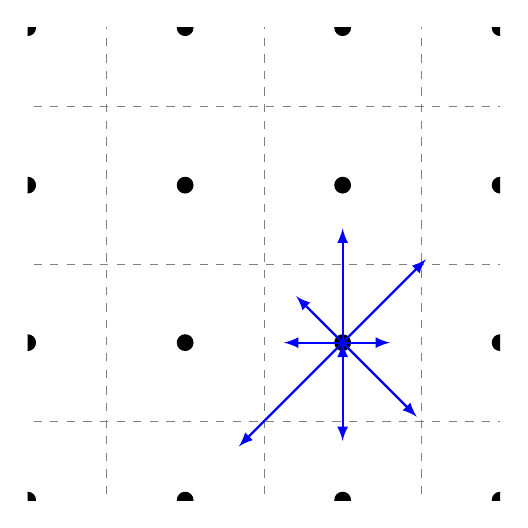
\begin{tikzpicture}
    \coordinate (Origin)   at (0,0);
    \coordinate (XAxisMin) at (-1,0);
    \coordinate (XAxisMax) at (5,0);
    \coordinate (YAxisMin) at (0,-1);
    \coordinate (YAxisMax) at (0,5);

    \clip (-1,-1) rectangle (5cm,5cm); % Clips the picture...
    \coordinate (Bone) at (0,2);
    \coordinate (Btwo) at (2,-2);
    \draw[style=help lines,dashed] (-14,-14) grid[step=2cm] (14,14);
    \foreach \x in {-7,-6,...,7}{% Two indices running over each
      \foreach \y in {-7,-6,...,7}{% node on the grid we have drawn 
        \node[draw,circle,inner sep=2pt,fill] at (1+2*\x,1+2*\y) {};
      }
    }
    \coordinate (exm)   at (3,1);
    \pgfmathsetseed{10}
    \foreach \x in {0, 1, -1}{
    	\foreach \y in {0, 1, -1}{
    		\pgfmathsetmacro{\ra}{0.5*rand+1}%
		    \draw [thick,-latex,blue] (exm)
			  --( $(exm) + (\x*\ra ,\y*\ra)$ ) node [] {};
	    }
    }
  \end{tikzpicture}
}
%
					\caption*{One collide step for a D2Q9-stencil}
				\end{figure}
			}
			\only<3>{
				\begin{figure}[htbp]
					\centering
					\setlength\figureheight{0.675\textheight} 
					\setlength\figurewidth{\figureheight} 
					\resizebox{\figurewidth}{\figureheight}{
 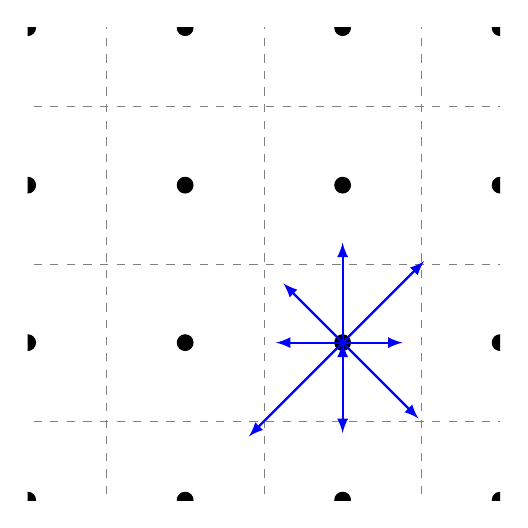
\begin{tikzpicture}
    \coordinate (Origin)   at (0,0);
    \coordinate (XAxisMin) at (-1,0);
    \coordinate (XAxisMax) at (5,0);
    \coordinate (YAxisMin) at (0,-1);
    \coordinate (YAxisMax) at (0,5);

    \clip (-1,-1) rectangle (5cm,5cm); % Clips the picture...
    \coordinate (Bone) at (0,2);
    \coordinate (Btwo) at (2,-2);
    \draw[style=help lines,dashed] (-14,-14) grid[step=2cm] (14,14);
    \foreach \x in {-7,-6,...,7}{% Two indices running over each
      \foreach \y in {-7,-6,...,7}{% node on the grid we have drawn 
        \node[draw,circle,inner sep=2pt,fill] at (1+2*\x,1+2*\y) {};
      }
    }
    \coordinate (exm)   at (3,1);
    \pgfmathsetseed{10}
    \foreach \x in {0, 1, -1}{
    	\foreach \y in {0, 1, -1}{
    		\pgfmathsetmacro{\ra}{0.3*rand+1}%
		    \draw [thick,-latex,blue] (exm)
			  --( $(exm) + (\x*\ra ,\y*\ra)$ ) node [] {};
	    }
    }
  \end{tikzpicture}
}
%
					\caption*{One collide step for a D2Q9-stencil}
				\end{figure}
			}
		\end{columns}
	\end{frame}
	\begin{frame}{Stream Step}
		\begin{columns}[t,totalwidth=\textwidth]
			\column{.4\linewidth}
			\centering
			\vspace{1cm}\\
			Particle distribution function $f_i$:
			\textcolor{red}{discrete in space and time}, continuous in probability values
			\column{.6\linewidth}
			\only<1>{
				\begin{figure}[htbp]
					\centering
					\setlength\figureheight{0.675\textheight} 
					\setlength\figurewidth{\figureheight} 
					\resizebox{\figurewidth}{\figureheight}{
 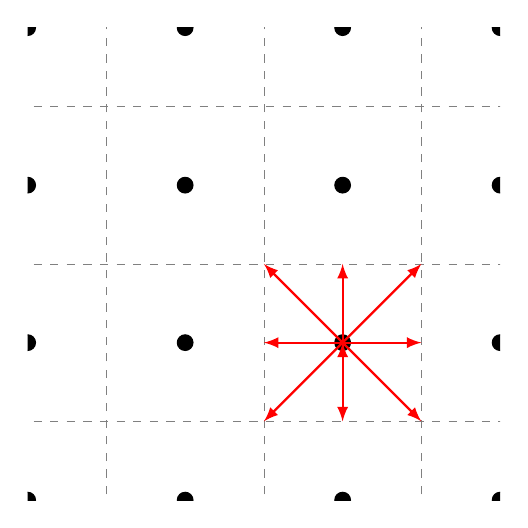
\begin{tikzpicture}
    \coordinate (Origin)   at (0,0);
    \coordinate (XAxisMin) at (-1,0);
    \coordinate (XAxisMax) at (5,0);
    \coordinate (YAxisMin) at (0,-1);
    \coordinate (YAxisMax) at (0,5);

    \clip (-1,-1) rectangle (5cm,5cm); % Clips the picture...
    \coordinate (Bone) at (0,2);
    \coordinate (Btwo) at (2,-2);
    \draw[style=help lines,dashed] (-14,-14) grid[step=2cm] (14,14);
    \foreach \x in {-7,-6,...,7}{% Two indices running over each
      \foreach \y in {-7,-6,...,7}{% node on the grid we have drawn 
        \node[draw,circle,inner sep=2pt,fill] at (1+2*\x,1+2*\y) {};
      }
    }
    \coordinate (exm)   at (3,1);
    \foreach \x in {0, 1, -1}{
    	\foreach \y in {0, 1, -1}{
		    \draw [thick,-latex,red] (exm)
			  --( $(exm) + (\x ,\y)$ ) node [] {};
	    }
    }
  \end{tikzpicture}
}
%
					\caption*{One stream step for a D2Q9-stencil}
				\end{figure}
			}
			\only<2>{
				\begin{figure}[htbp]
					\centering
					\setlength\figureheight{0.675\textheight} 
					\setlength\figurewidth{\figureheight} 
					\resizebox{\figurewidth}{\figureheight}{
 \begin{tikzpicture}
    \coordinate (Origin)   at (0,0);
    \coordinate (XAxisMin) at (-1,0);
    \coordinate (XAxisMax) at (5,0);
    \coordinate (YAxisMin) at (0,-1);
    \coordinate (YAxisMax) at (0,5);
    \clip (-1,-1) rectangle (5cm,5cm); % Clips the picture...
    \coordinate (Bone) at (0,2);
    \coordinate (Btwo) at (2,-2);
    \draw[style=help lines,dashed] (-14,-14) grid[step=2cm] (14,14);
    \foreach \x in {-7,-6,...,7}{% Two indices running over each
      \foreach \y in {-7,-6,...,7}{% node on the grid we have drawn 
        \node[draw,circle,inner sep=2pt,fill] at (1+2*\x,1+2*\y) {};
      }
    }
    \coordinate (exm)   at (3,1);
    \foreach \x in {0, 1, -1}{
    	\foreach \y in {0, 1, -1}{
    		\coordinate (neigh)   at ($(exm) + 2*(\x ,\y)$);
		    \draw [thick,-latex,red] (neigh)
			  --( $(neigh) + (\x ,\y)$ ) node [] {};
	    }
    }
  \end{tikzpicture}
}
%
					\caption*{One stream step for a D2Q9-stencil}
				\end{figure}
			}
		\end{columns}
	\end{frame}

	
	\begin{frame}{The Lattice Boltzmann Equation}

			{...is what we get when we apply both steps:}
			\begin{align*}	
				\textcolor{red}{f_i(\bm{x} + \bm{c_i}\Delta t, t + \Delta t)} = \textcolor{blue}{f_i(\bm{x}, t) + \Omega_i(\bm{x}, t)}
			\end{align*}
			\newline
			\only<2-4>{
			With collision operator $\Omega_i(\bm{x}, t)$, e.g.:
			\begin{itemize}
				\item BGK: $\Omega (f)={\frac {1}{\tau}}(f_{i}^{\text{eq}}-f_{i}) = \omega (f_{i}^{\text{eq}}-f_{i}) $
				\item TRT: is often nicer but needs more formulas $\rightarrow$ please look up
			\end{itemize}
			\par\bigskip
			\only<3-4>{
			and the equilibrium particle distribution function $f_{i}^{\text{eq}} = w_{i}\rho \left(1+{\frac {{\vec {e}}_{i}{\vec {u}}}{c_{s}^{2}}}+{\frac {({\vec {e}}_{i}{\vec {u}})^{2}}{2c_{s}^{4}}}-{\frac {{\vec {u}}^{2}}{2c_{s}^{2}}}\right)$
			\only<4->{	
			
				\hfill $w_0 = \frac{4}{9}, w_{1,2,3,4} = \frac{1}{9}, w_{5,6,7,8} = \frac{1}{36}$ for D2Q9 
			}
			}
			}
			\only<5 | handout:0>{Cf. Boltzmann Equation
				\begin{align*}%stolen from wikipedia
					{{\frac {\partial f}{\partial t}}+{\frac {\bm {p} }{m}}\cdot \nabla f=\left({\frac {\partial f}{\partial t}}\right)_{ {coll} }}
				\end{align*}
			}
		%B E
		%Collision operators
	\end{frame}
	
	\begin{frame}{Moments - the Interesting Outputs in LBM}
		Density and velocity are given locally
		
		\begin{align*}
			\rho(\bm{x}, t) = \sum_i f_i(\bm{x},t)
		\end{align*}
		\begin{align*}
			\rho \bm{u}(\bm{x}, t) = \sum_i \bm{c_i} f_i(\bm{x},t)
		\end{align*}
	\end{frame}
	
	\begin{frame}{Nondimensionalization -- setting the step size}
		= Normalization in the three physical dimensions time, space, mass \newline
		\par\bigskip
		\pause
		Usual choice:
		\begin{align*}
			\Delta x^*  = 1 = C_x \cdot \Delta x\\ 
			\Delta t^* = 1 = C_t \cdot \Delta t\\ 
			\Delta \rho^* = 1 = C_\rho \cdot \Delta \rho\\ 
		\end{align*}
		\pause
		The kinematic velocity in lattice units is directly linked to $\omega$ or $\tau$: \pause
		\begin{align*}
			\nu^* = (\tau - 0.5 ) c_{s}^{2} = (\frac{1}{\omega} - 0.5 ) c_{s}^{2}, \,\,\,\,
			\pause
			c_{s}^{2} = \frac{1}{3}\\
		\end{align*}
		\centering
		$\Rightarrow 0.5 < \tau$  ... and not much larger than 1!
		\newline\par\smallskip
	\end{frame}
	
	\begin{frame}{LBM -- advantages and disadvantages}
		\centering
		\begin{tabular}{c c}
			\bfseries advantages & \bfseries disadvantages \\\hline
			\begin{minipage}{0.4\linewidth}
				\vspace{1ex}
				\begin{itemize}
					\pause
					\item (moderately) easy to implement
					\pause
					\item easy to parallelize
					\pause
					\item yields Navier-Stokes (by Chapman-Enskog analysis)
					\pause
					\item Galilean invariance
					\pause
				\end{itemize}
			\end{minipage}
			&\begin{minipage}{0.4\linewidth}
				\vspace{1ex}
				\begin{itemize}
					\item needs parameter fine-tuning
					\pause
					\item explicit scheme $\rightarrow$  may need fine time resolution for stability, compared to other CFD methods
				\end{itemize}
			\end{minipage}
		\end{tabular}
	\end{frame}
	
\end{section}


  { % Questions?
    \setbeamertemplate{footline}{}
    \begin{frame}[c,noframenumbering]
      \begin{center}
        Thanks for listening.\\
        {\bf Any questions?}
      \end{center}
    \end{frame}

    % References
    \section*{References}
    %TODO List all references or remove slides - I would only mention the references that are actually used for our presentation, my references are already there (Christoph)
    \begin{frame}[noframenumbering]{References}
      \printbibliography
    \end{frame}
  }
\end{document}
